\section{Модель данных}

Для интеграции подсистемы аутентификации с применением ПЦКД в корпоративную
информационую систему необходима база данных для хранения пользовательской
информации и обеспечения функционирования серверных модулей. На
рисунке~\ref{ris:3.5} представлейна минимальная схема базы данных, необходимая
для успешной интеграции данной подсистемы. Предложенная модель построена по
принципу <<необходимости, но недостаточности>> и может быть расширена другими
сущностями, необходимыми для работы конкретной корпоративной информационной
системы.

\begin{figure}[h!]
\center{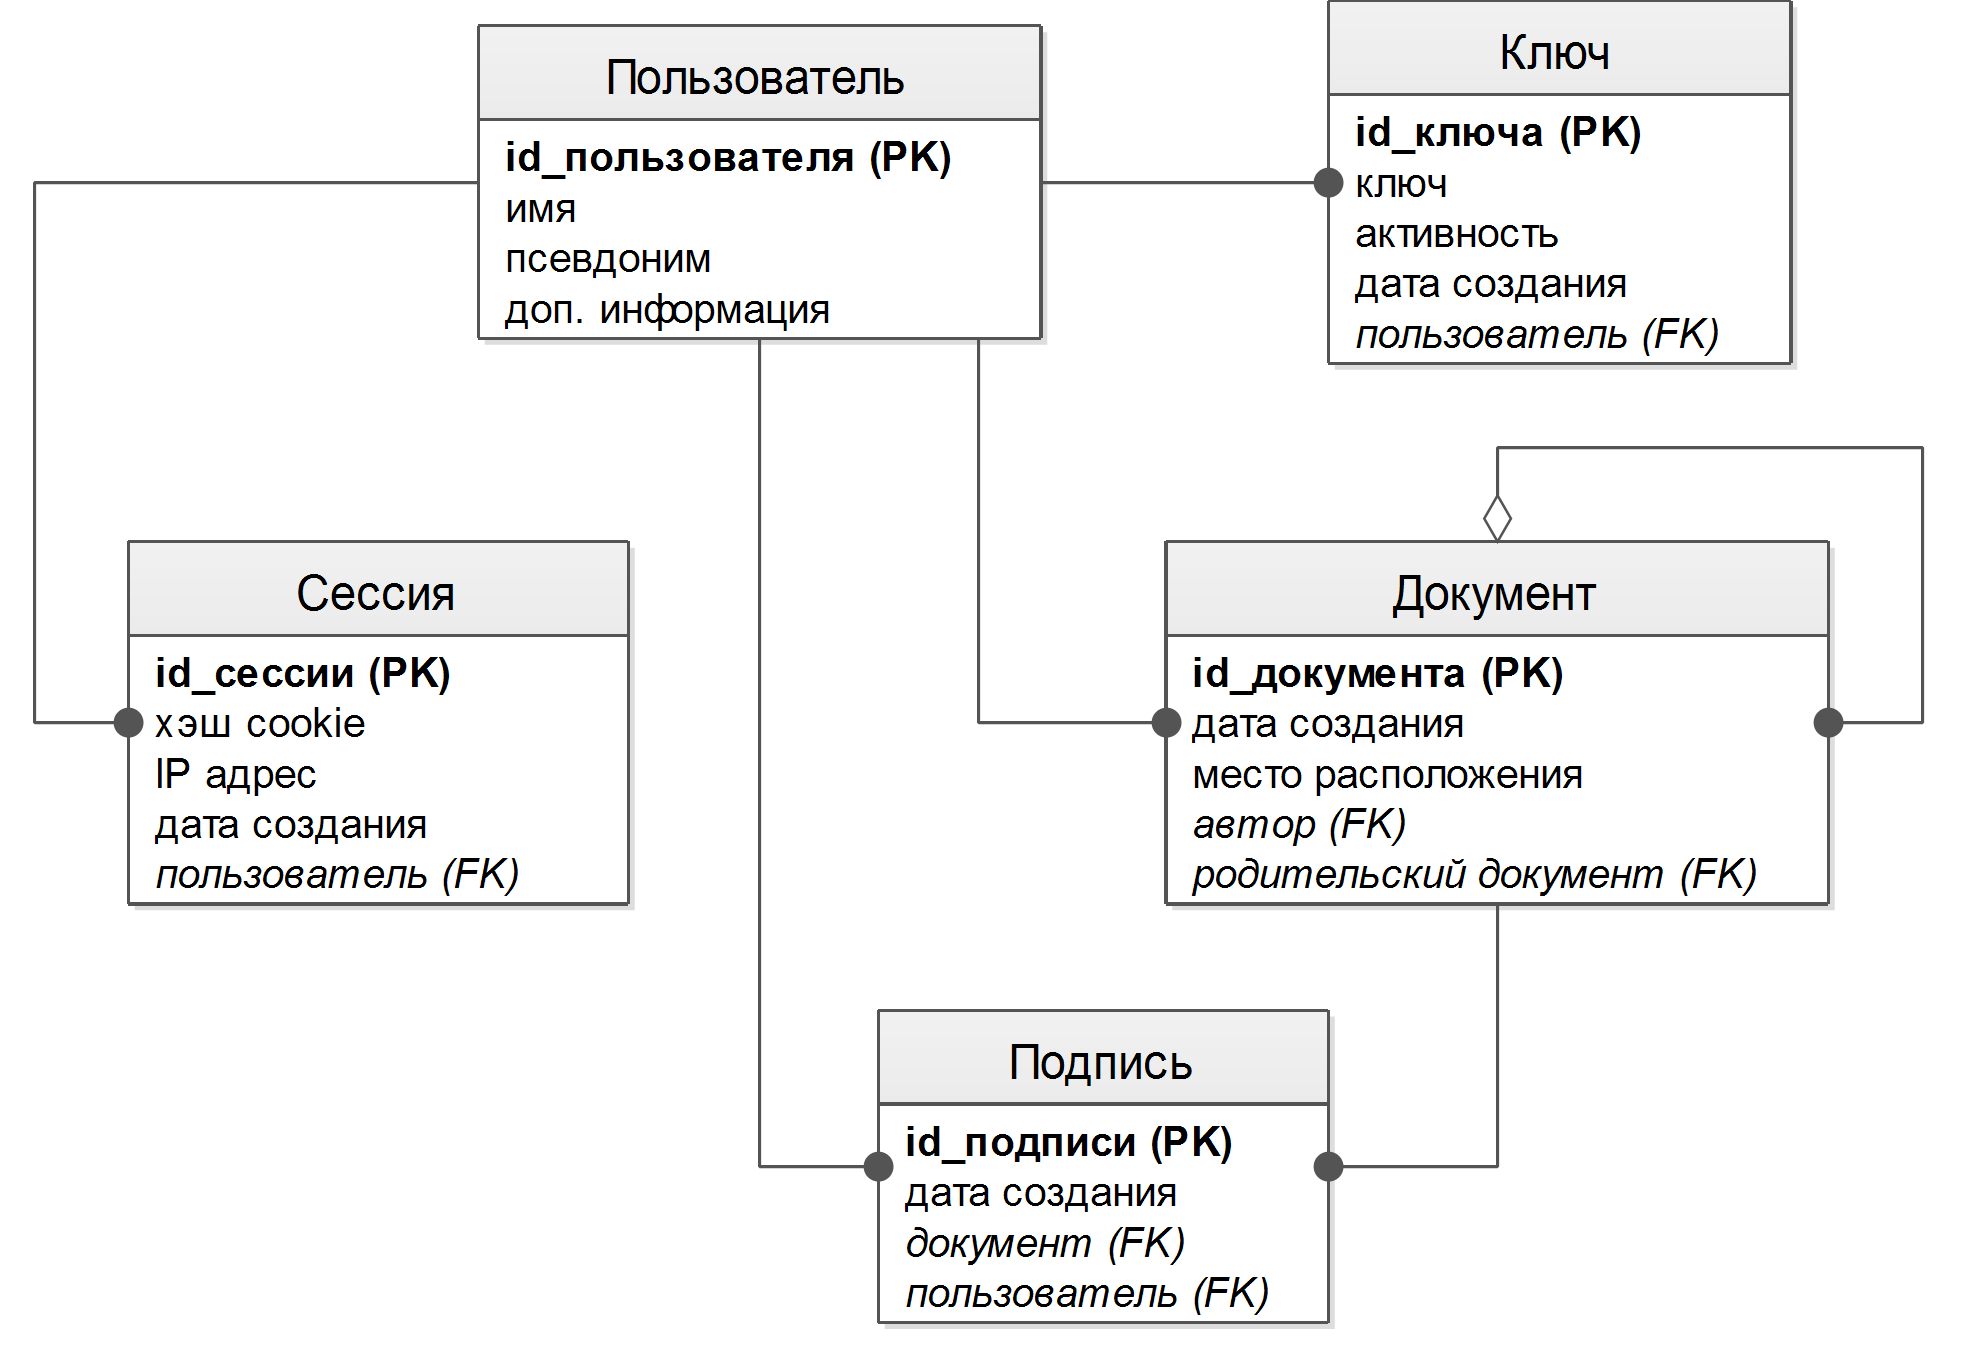
\includegraphics[width=1\linewidth]{3-5}}
\caption{Концептуальная модель данных}
\label{ris:3.5}
\end{figure}

Центральной сущностью концептуальной модели данных является
сущность <<Пользователь>>, так как от нее отталкиваются другие объекты.
Данная сущность описывает пользователя системы и имеет атрибуты:
\begin{itemize}
  \item идентификатор пользователя -- первичный ключ;
  \item имя;
  \item дополнительная информация, характеризующая пользователя (телефонный
  номер, адрес электронной почты).
\end{itemize}

Сущность <<Пользователь>>, теоретически, может быть позаимствована из уже
существующей базы данных, установив соответствие между идентификатором
пользователя и связанными с ним объектами.

Сущность <<Ключ>> описывает информацию, касаемую секретных ключей и имеет
следующие атрибуты:

\begin{itemize}
  \item идентификатор ключа -- первичный ключ;
  \item ключ;
  \item активность -- указывает на возможность использования данного ключа;
  \item дата создания.
\end{itemize}

Каждый пользователь может иметь неограниченное количество ключей, но в
конкретный момент активным может быть только один. Поэтому должен быть
предусмотрен триггер, ведущий слежение за активностью ключей, а так же их
деактивацию при истечении срока службы.

Сущность <<Сессия>> описывает информацию, необходимую для поддержания
пользовательского сеанса. Так же ее можно использовать для ведения учета
посещаемости пользователей (аккаунтинг).

Сущность <<Документ>> описывает файлы, размещаемые пользователем для
осуществления электронного документаоборота. Данная сущность имеет следующие
атрибуты:

\begin{itemize}
  \item идентификатор документа -- первичный ключ;
  \item место расположения -- указывает на адрес размещения файла;
  \item дата создания.
\end{itemize}

\begin{algorithm}[h!]
\floatname{algorithm}{Алгоритм}                 % enter the algorithm
\caption{Функционирование ПЦКД}          % give the algorithm a caption
\label{alg:1}     
\small                      % and a label for \ref{} commands later in the
% document
\begin{algorithmic}[1]      
\State $n \gets 64$ \Comment{размер буфера обмена в байтах}
\State $page \gets 1024$ \Comment{page -- адресс памяти}
\Loop
  \State $iBuf \gets $ \Call{Чтение входного буфера}{void}
  \If{$iBuf$ НЕ пустой}
    \If{$iBuf[0] = 1$} \Comment{Вычисление сигнатуры}
      \State $pBuf \gets $ \Call{Чтение из внутренней flash-памяти}{page}
      \State $alg \gets pBuf, id \gets pBuf, secret \gets bBuf, message \gets
      pbuf$ \Comment{Парсинг pBuf: alg -- алгоритм, id -- идентификатор
      пользователя а системе, secret -- закытый ключ, message -- входное сообщение}
      \State $tBuf \gets$ \Call {Вычисление сигнатуры}{message, secret, alg}
      \Comment{В соответствии с заданным алгоритмом шифрования}
      \State $oBuf \gets tBuf + id$ \Comment{Конкатенация массивов}
    \EndIf    
    
    \If{$iBuf[0] = 2$} \Comment{Запись параметров в память}
      
      \State $pBuf[0..n-1] \gets iBuf[1..n]$
      \State $pBuf \gets $ \Call{Расшифровка}{pBuf, key} \Comment{key -- ключ
      расшифровки } \State \Call{Запись во внутреннюю flash-память}{pBuf,
      page}
      \State $pBuf[0..n] \gets 0$ \Comment{Тестирование записи}
      \State $pBuf \gets $ \Call{Чтение из внутренней flash-памяти}{page}
      \State $oBuf \gets pBuf$
    \EndIf
    
    \State Запись в выходной буфер ($oBuf$)
  \EndIf
\EndLoop

\end{algorithmic}
\end{algorithm}

Данная сущность является рекурсивной. Это исходит из того факта, что каждый
документ может иметь потомков, то есть документов, полученных на основе данного,
путем изменения и редактирования.

Сущность <<Подпись>> описывает информацию, предназначенную для подтверждения
подлинности документов. Данные для данной сущности поступают от клиентских
компонентов системы и извлекаются в процессе верификации.
